% 本ファイルは \texttt{python -m analytics.future\_directions\_analysis} または \texttt{run\_analysis.py} 実行時に上書きされる。
% auto-generated by analytics/future_directions_analysis.py
\subsection{提案の図解と proxy 感度}
\label{sec:future_figures}
「今後の方針」の箇条書きと「追加で欲しいデータ」を、パイロット割付・90日副次・粗利未観測時の感度・データギャップとして図示する。
いずれも\textbf{設計・監査用の補助}であり、因果効果の確定は無作為化試験に委ねる。

\begin{figure}[!htbp]
  \centering
  \begin{subfigure}[t]{0.49\linewidth}
    \centering
    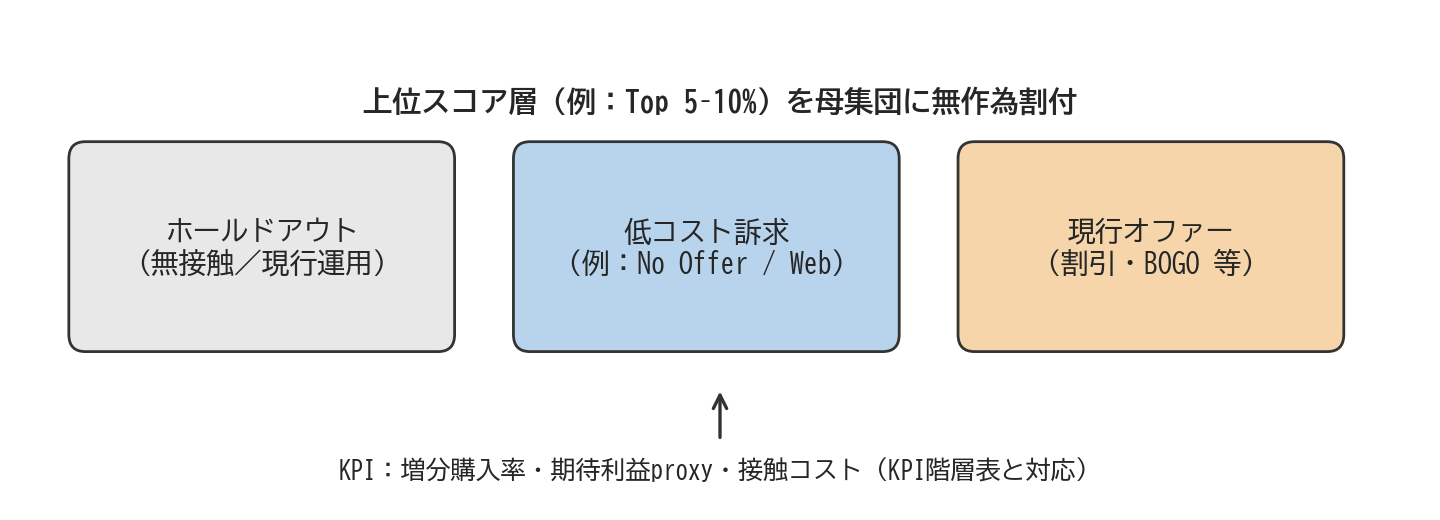
\includegraphics[width=\linewidth]{../figures/improvements/future_pilot_arm_schematic.png}
    \caption{上位スコア層を母集団とした\textbf{3臂}（低コスト訴求・現行オファー・ホールドアウト）。因子はチャネル等に拡張可。}
    \label{fig:future_pilot_arms}
  \end{subfigure}\hfill
  \begin{subfigure}[t]{0.49\linewidth}
    \centering
    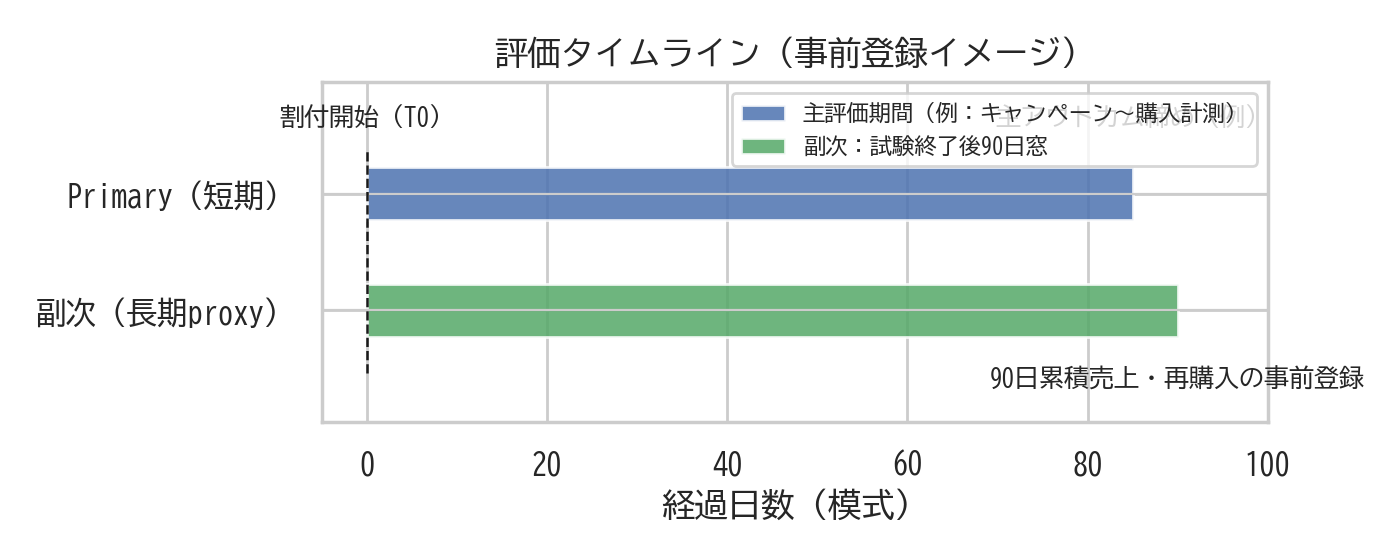
\includegraphics[width=\linewidth]{../figures/improvements/future_kpi_timeline_90d.png}
    \caption{主アウトカム（短期）と事前登録した\textbf{90日}副次（累積売上・再購入等）。日付は組織で調整。}
    \label{fig:future_kpi_timeline}
  \end{subfigure}
  \caption{パイロット割付（左）と評価タイムライン（右）の模式}
  \label{fig:future_pilot_and_timeline}
\end{figure}

\begin{figure}[!htbp]
  \centering
  \begin{subfigure}[t]{0.48\linewidth}
    \centering
    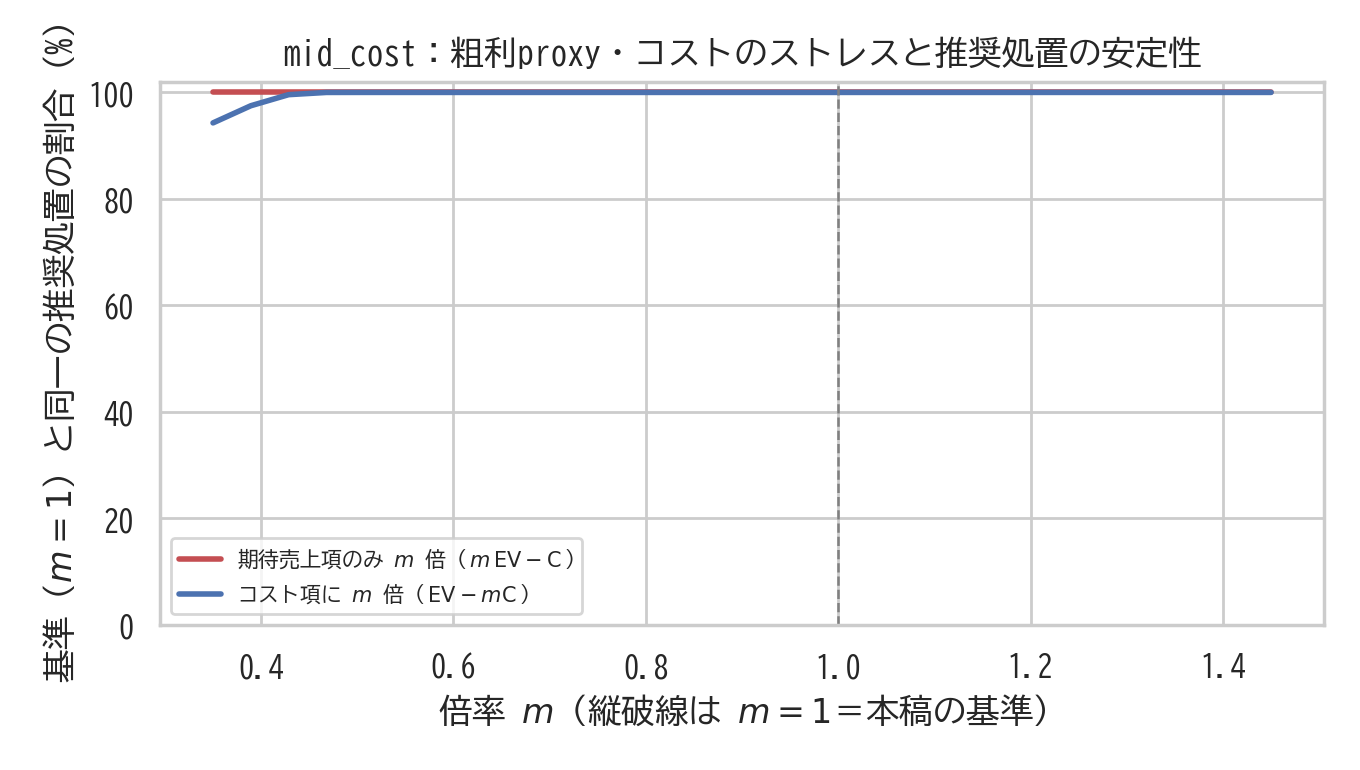
\includegraphics[width=\linewidth]{../figures/improvements/future_profit_margin_sensitivity.png}
    \caption{\textbf{真の粗利・返品・原価・実コスト}が未観測のとき、オフライン推奨は感度が大きい。
    \textbf{赤}は期待売上項だけ $m$ 倍（$m\,\mathrm{EV}-\mathrm{C}$）---{}粗利proxyが薄い・転換時の価値が過大評価のイメージ。
    \textbf{青}はコスト項に $m$ 倍（$\mathrm{EV}-m\mathrm{C}$）---{}インセンティブ・接触コストが想定より重い／軽いストレス。
    なお $(\mathrm{EV}-\mathrm{C})$ 全体に同一の $m>0$ を掛けても argmax は変わらない（本図には描かない）。
    数値は \texttt{artifacts/future\_margin\_sensitivity.csv}。}
    \label{fig:future_margin_sens}
  \end{subfigure}\hfill
  \begin{subfigure}[t]{0.48\linewidth}
    \centering
    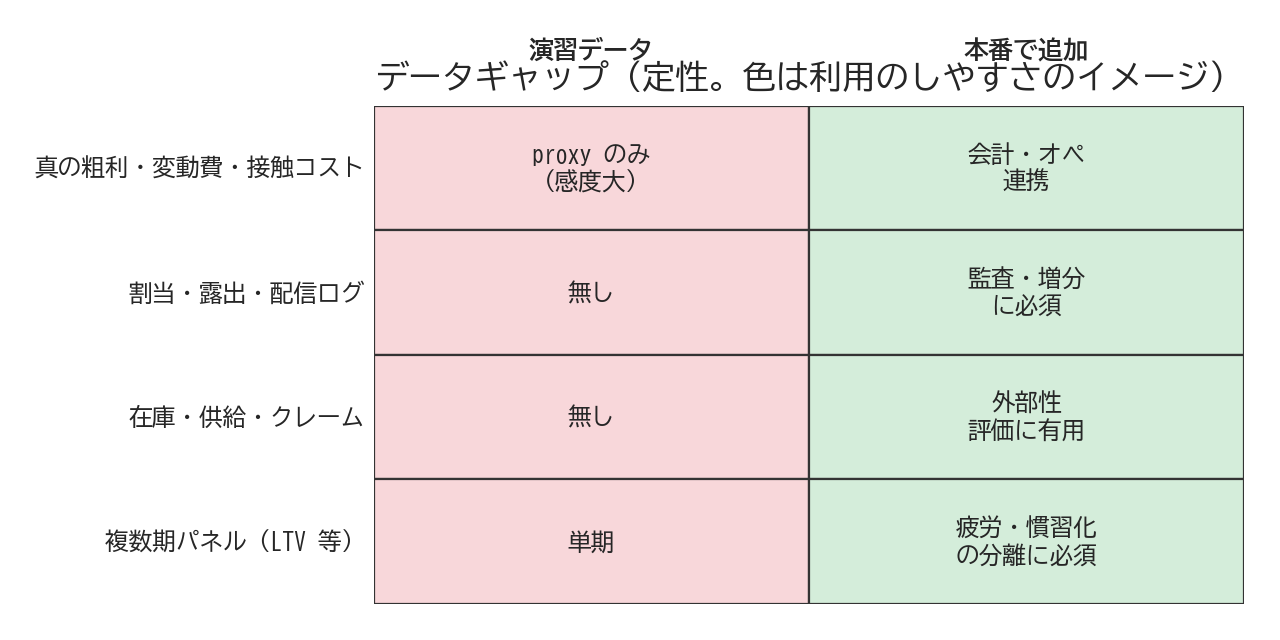
\includegraphics[width=\linewidth]{../figures/improvements/future_data_gap_matrix.png}
    \caption{演習データに無い要素と、本番で揃えるとよいデータ（追加で欲しいデータの対応表・定性）。}
    \label{fig:future_data_gap}
  \end{subfigure}
  \caption{粗利・コスト未観測時のオフライン推奨感度（左）とデータギャップの定性マトリクス（右）}
\end{figure}

\FloatBarrier
